% Options for packages loaded elsewhere
\PassOptionsToPackage{unicode}{hyperref}
\PassOptionsToPackage{hyphens}{url}
%
\documentclass[
  letterpaper,
  ignorenonframetext,
  aspectratio=43,
  handout,
  12pt]{beamer}
\usepackage{pgfpages}
\setbeamertemplate{caption}[numbered]
\setbeamertemplate{caption label separator}{: }
\setbeamercolor{caption name}{fg=normal text.fg}
\beamertemplatenavigationsymbolsempty
% Prevent slide breaks in the middle of a paragraph
\widowpenalties 1 10000
\raggedbottom
\setbeamertemplate{part page}{
  \centering
  \begin{beamercolorbox}[sep=16pt,center]{part title}
    \usebeamerfont{part title}\insertpart\par
  \end{beamercolorbox}
}
\setbeamertemplate{section page}{
  \centering
  \begin{beamercolorbox}[sep=12pt,center]{part title}
    \usebeamerfont{section title}\insertsection\par
  \end{beamercolorbox}
}
\setbeamertemplate{subsection page}{
  \centering
  \begin{beamercolorbox}[sep=8pt,center]{part title}
    \usebeamerfont{subsection title}\insertsubsection\par
  \end{beamercolorbox}
}
\AtBeginPart{
  \frame{\partpage}
}
\AtBeginSection{
  \ifbibliography
  \else
    \frame{\sectionpage}
  \fi
}
\AtBeginSubsection{
  \frame{\subsectionpage}
}
\usepackage{amsmath,amssymb}
\usepackage{lmodern}
\usepackage{iftex}
\ifPDFTeX
  \usepackage[T1]{fontenc}
  \usepackage[utf8]{inputenc}
  \usepackage{textcomp} % provide euro and other symbols
\else % if luatex or xetex
  \usepackage{unicode-math}
  \defaultfontfeatures{Scale=MatchLowercase}
  \defaultfontfeatures[\rmfamily]{Ligatures=TeX,Scale=1}
\fi
\usetheme[]{metropolis}
% Use upquote if available, for straight quotes in verbatim environments
\IfFileExists{upquote.sty}{\usepackage{upquote}}{}
\IfFileExists{microtype.sty}{% use microtype if available
  \usepackage[]{microtype}
  \UseMicrotypeSet[protrusion]{basicmath} % disable protrusion for tt fonts
}{}
\makeatletter
\@ifundefined{KOMAClassName}{% if non-KOMA class
  \IfFileExists{parskip.sty}{%
    \usepackage{parskip}
  }{% else
    \setlength{\parindent}{0pt}
    \setlength{\parskip}{6pt plus 2pt minus 1pt}}
}{% if KOMA class
  \KOMAoptions{parskip=half}}
\makeatother
\usepackage{xcolor}
\IfFileExists{xurl.sty}{\usepackage{xurl}}{} % add URL line breaks if available
\IfFileExists{bookmark.sty}{\usepackage{bookmark}}{\usepackage{hyperref}}
\hypersetup{
  hidelinks,
  pdfcreator={LaTeX via pandoc}}
\urlstyle{same} % disable monospaced font for URLs
\newif\ifbibliography
\usepackage{graphicx}
\makeatletter
\def\maxwidth{\ifdim\Gin@nat@width>\linewidth\linewidth\else\Gin@nat@width\fi}
\def\maxheight{\ifdim\Gin@nat@height>\textheight\textheight\else\Gin@nat@height\fi}
\makeatother
% Scale images if necessary, so that they will not overflow the page
% margins by default, and it is still possible to overwrite the defaults
% using explicit options in \includegraphics[width, height, ...]{}
\setkeys{Gin}{width=\maxwidth,height=\maxheight,keepaspectratio}
% Set default figure placement to htbp
\makeatletter
\def\fps@figure{htbp}
\makeatother
% Make links footnotes instead of hotlinks:
\DeclareRobustCommand{\href}[2]{#2\footnote{\url{#1}}}
\setlength{\emergencystretch}{3em} % prevent overfull lines
\providecommand{\tightlist}{%
  \setlength{\itemsep}{0pt}\setlength{\parskip}{0pt}}
\setcounter{secnumdepth}{-\maxdimen} % remove section numbering
\usepackage{pgfpages}
\pgfpagesuselayout{2 on 1}
\providecommand{\tightlist}{%
\setlength{\itemsep}{0pt}\setlength{\parskip}{0pt}}
\makeatletter
\makeatother
\let\Oldincludegraphics\includegraphics
\renewcommand{\includegraphics}[2][]{\Oldincludegraphics[width=\textwidth,height=0.7\textheight,keepaspectratio]{#2}}
\ifLuaTeX
  \usepackage{selnolig}  % disable illegal ligatures
\fi

\author{}
\date{}

\begin{document}

\begin{frame}{Theory of Elasticity}
\protect\hypertarget{theory-of-elasticity}{}
Dr.~Nicholas Smith

Wichita State University, Department of Aerospace Engineering October 7,
2021
\end{frame}

\begin{frame}{upcoming schedule}
\protect\hypertarget{upcoming-schedule}{}
\begin{itemize}
\tightlist
\item
  Oct 7 - Exam 2 Review
\item
  Oct 8 - Homework 4 Self-grade Due, Homework 5 Due
\item
  (Oct 12) - Fall Break (No Class)
\item
  Oct 14 - Exam 2
\item
  Oct 19 - Strain Energy
\item
  Oct 21 - Virtual Work
\end{itemize}
\end{frame}

\begin{frame}{outline}
\protect\hypertarget{outline}{}
\begin{itemize}
\tightlist
\item
  exam
\item
  group problems
\item
  stress and equilibrium
\item
  material behavior
\item
  problem formulation
\end{itemize}
\end{frame}

\hypertarget{exam}{%
\section{exam}\label{exam}}

\begin{frame}{exam format}
\protect\hypertarget{exam-format}{}
\begin{itemize}
\tightlist
\item
  Similar format to last exam
\item
  Three problems
\item
  Focus on organizing your work clearly to maximize partial credit
\end{itemize}
\end{frame}

\hypertarget{group-problems}{%
\section{group problems}\label{group-problems}}

\begin{frame}{problem one - thermoelasticity}
\protect\hypertarget{problem-one---thermoelasticity}{}
As a first-order model of the problem of freezing water in a glass
bottle, we treat water as a thermoelastic solid and the glass as a fixed
boundary. Find the stress and strain field in the water as a function of
the elastic properties (\(E,\nu\)) and the coefficient of thermal
expansion (\(\alpha\)).
\end{frame}

\begin{frame}{problem two - inverse solution}
\protect\hypertarget{problem-two---inverse-solution}{}
Consider the stress field

\[ \sigma = \begin{bmatrix} Ay & 0 & 0 \ 0 & 0 & 0 \ 0 & 0 & 0 \end{bmatrix}  \]

Show that this is a valid solution to an elasticity problem. What
problem does it solve?
\end{frame}

\begin{frame}{problem three - semi-inverse}
\protect\hypertarget{problem-three---semi-inverse}{}
To solve the problem of torsion in prismatic bars we consider the
displacement field

\[ u = -\alpha y z, \qquad v = -\alpha x z, \qquad w = w(x,y) \]

Solve this problem using the boundary conditions for a solid square
cross-section.
\end{frame}

\hypertarget{stress-and-equilibrium}{%
\section{stress and equilibrium}\label{stress-and-equilibrium}}

\begin{frame}{topics}
\protect\hypertarget{topics}{}
\begin{itemize}
\tightlist
\item
  Traction
\item
  Stress transformation
\item
  Principal stress
\item
  Equilibrium
\end{itemize}
\end{frame}

\begin{frame}{derivations}
\protect\hypertarget{derivations}{}
\begin{itemize}
\tightlist
\item
  Cauchy's stress theorem
\item
  Max shear stress for plane stress
\item
  Mohr's circle
\end{itemize}
\end{frame}

\begin{frame}{stress tensor}
\protect\hypertarget{stress-tensor}{}
\begin{columns}[T]
\begin{column}{0.5\textwidth}
\begin{itemize}
\tightlist
\item
  To simplify the notation, we introduce the stress tensor
\end{itemize}

\[\sigma_{ij} = t_j^{(\hat{e}_i)}\]
\end{column}

\begin{column}{0.5\textwidth}
\begin{figure}
\centering
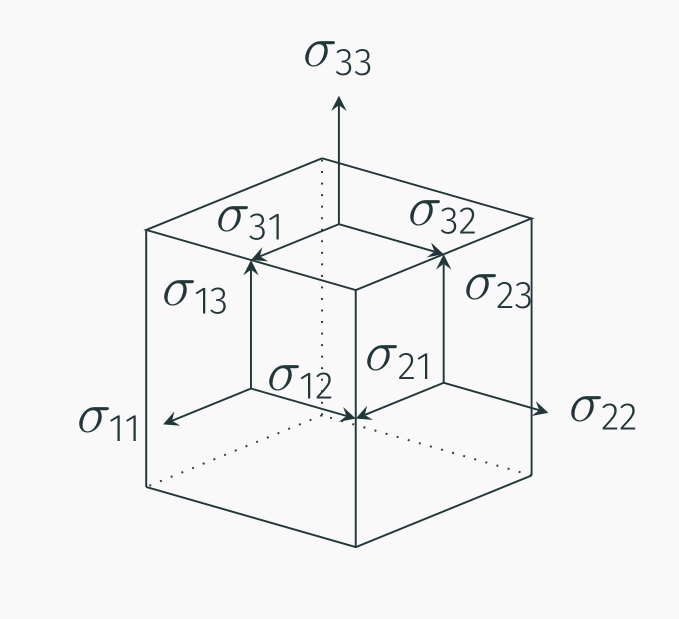
\includegraphics{../images/stress-cube.png}
\caption{stress tensor illustrated on a cube}
\end{figure}
\end{column}
\end{columns}
\end{frame}

\begin{frame}{traction}
\protect\hypertarget{traction}{}
\begin{itemize}
\tightlist
\item
  We can find some interesting information about the traction vector by
  considering an arbitrary tetrahedron with some traction
  \(\hat{t}^{(n)}\) applied to the surface
\end{itemize}
\end{frame}

\begin{frame}{traction}
\protect\hypertarget{traction-1}{}
\begin{itemize}
\tightlist
\item
  If we consider the balance of forces in the \(x_1\)-direction
\end{itemize}

`\$t\_1 dA - \sigma\emph{\{11\} dA\_1 - \sigma}\{21\} dA\_2 -
\sigma\_\{31\}dA\_3 + b\_1 \rho dV = 0\textbackslash{]}

\begin{itemize}
\tightlist
\item
  The area components are:
\end{itemize}

\[\begin{aligned}
    dA_1 &= n_1 dA\\
    dA_2 &= n_2 dA\\
    dA_3 &= n_3 dA\\
\end{aligned}\]

\begin{itemize}
\tightlist
\item
  And \(dV = \frac{1}{3}h dA\).
\end{itemize}
\end{frame}

\begin{frame}{traction}
\protect\hypertarget{traction-2}{}
\[t_1 dA - \sigma_{11} n_1 dA - \sigma_{21} n_2 dA - \sigma_{31} n_3 dA + b_1 \rho \frac{1}{3}h dA = 0\]

\begin{itemize}
\tightlist
\item
  If we let \(h \to 0\) and divide by \emph{dA}
\end{itemize}

\[t_1 = \sigma_{11}n_1 + \sigma_{21}n_2 + \sigma_{31}n_3\]

\begin{itemize}
\tightlist
\item
  We can write this in index notation as
\end{itemize}

\[t_1 = \sigma_{i1}n_i\]
\end{frame}

\begin{frame}{traction}
\protect\hypertarget{traction-3}{}
\begin{itemize}
\tightlist
\item
  We find, similarly
\end{itemize}

\[\begin{aligned}
    t_2 &= \sigma_{i2} n_i\\
    t_3 &= \sigma_{i3} n_i\\
\end{aligned}\]
\end{frame}

\begin{frame}{traction}
\protect\hypertarget{traction-4}{}
\begin{itemize}
\tightlist
\item
  We can further combine these results in index notation as
\end{itemize}

\[t_j = \sigma_{ij}n_i\]

\begin{itemize}
\tightlist
\item
  This means with knowledge of the nine components of \(\sigma_{ij}\),
  we can find the traction vector at any point on any surface
\end{itemize}
\end{frame}

\begin{frame}{maximum shear stress}
\protect\hypertarget{maximum-shear-stress}{}
\begin{itemize}
\tightlist
\item
  For plane stress problems, we can also use the stress transformation
  equations to find the maximum shear stress
\item
  We desire to maximize this equation:
\end{itemize}

\[\tau^\prime_{xy} = \frac{\sigma_y - \sigma_x}{2}\sin 2\theta + \tau_{xy} \cos 2\theta\]
\end{frame}

\begin{frame}{maximum shear stress}
\protect\hypertarget{maximum-shear-stress-1}{}
\begin{itemize}
\tightlist
\item
  Taking the derivative with respect to \(\theta\) gives
\end{itemize}

\[\frac{\partial}{\partial \theta} (\tau^\prime_{xy}) = (\sigma_y-\sigma_x)\cos 2\theta - 2\tau_{xy} \sin 2\theta = 0\]

\begin{itemize}
\tightlist
\item
  Which we can use to find 2\emph{θ}
\end{itemize}

\[2\theta = \tan ^{-1} \left(\frac{(\sigma_y-\sigma_x)}{2\tau_{xy}}\right)\]
\end{frame}

\begin{frame}{maximum shear stress}
\protect\hypertarget{maximum-shear-stress-2}{}
\begin{itemize}
\tightlist
\item
  Substituting back into the original equation gives
\end{itemize}

\[\tau^\prime_{max} = \frac{\sigma_y - \sigma_x}{2}\sin \left[\tan ^{-1} \left(\frac{(\sigma_y-\sigma_x)}{2\tau_{xy}}\right)\right] + \tau_{xy} \cos \left[\tan ^{-1} \left(\frac{(\sigma_y-\sigma_x)}{2\tau_{xy}}\right)\right]\]

\begin{itemize}
\tightlist
\item
  Note that
\end{itemize}

\[\begin{aligned}
    \sin (\tan ^{-1} (x)) &= \frac{x}{\sqrt{1+x^2}}\\
    \cos (\tan ^{-1} (x)) &= \frac{1}{\sqrt{1+x^2}}\\
\end{aligned}\]
\end{frame}

\begin{frame}{maximum shear stress}
\protect\hypertarget{maximum-shear-stress-3}{}
\begin{itemize}
\tightlist
\item
  We note that
\end{itemize}

\[\sqrt{1+ \left(\frac{\sigma_y - \sigma_x}{2 \tau_{xy}}\right)^2} = \frac{\sqrt{(\sigma_y-\sigma_x)^2+4\tau_{xy}^2}}{2\tau_{xy}}\]

\begin{itemize}
\tightlist
\item
  And thus we find
\end{itemize}

\[\tau_{max} = \frac{(\sigma_y-\sigma_x)^2}{2 \sqrt{(\sigma_y-\sigma_x)^2+4\tau_{xy}^2}} + \frac{4\tau_{xy}^2}{2 \sqrt{(\sigma_y-\sigma_x)^2+4\tau_{xy}^2}}\]
\end{frame}

\begin{frame}{maximum shear stress}
\protect\hypertarget{maximum-shear-stress-4}{}
\begin{itemize}
\tightlist
\item
  Adding the terms and simplifying, we find
\end{itemize}

\[\tau_{max} = \sqrt{\left(\frac{\sigma_y-\sigma_x}{2}\right)^2+\tau_{xy}^2}\]
\end{frame}

\begin{frame}{tractions}
\protect\hypertarget{tractions}{}
\begin{columns}[T]
\begin{column}{0.5\textwidth}
\begin{itemize}
\tightlist
\item
  We can use what we know about principal values to find some
  interesting things about the tractions
\item
  Consider the traction vector on an arbitrary internal face, and
  decompose into Normal and Shear components.
\end{itemize}
\end{column}

\begin{column}{0.5\textwidth}
\begin{figure}
\centering
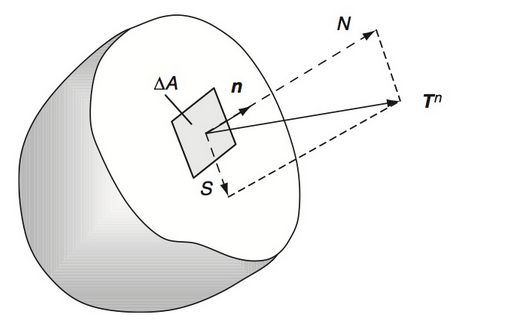
\includegraphics{../images/potato.PNG}
\caption{arbitrary body with arbitrary loading applied}
\end{figure}
\end{column}
\end{columns}
\end{frame}

\begin{frame}{tractions}
\protect\hypertarget{tractions-1}{}
\begin{itemize}
\tightlist
\item
  The normal component can be found using the dot product
\end{itemize}

\[N = \hat{T}^n \cdot \hat{n}\]

\begin{itemize}
\tightlist
\item
  The shear component can be found using the Pythagorean theorem
\end{itemize}

\[S^2 = |\hat{T}^n|^2 - N^2\]
\end{frame}

\begin{frame}{tractions}
\protect\hypertarget{tractions-2}{}
\begin{itemize}
\tightlist
\item
  We now use the stress tensor in the principal direction to simplify
  the calculations
\end{itemize}

\[\begin{aligned}
    N &= \hat{T}^n \cdot \hat{n}\\
    &= T^n_i n_i \\
    &= \sigma_{ji} n_j n_i\\
    &= \sigma_1 n_1^2 + \sigma_2 n_2^2 + \sigma_3 n_3^2
\end{aligned}\]
\end{frame}

\begin{frame}{tractions}
\protect\hypertarget{tractions-3}{}
\begin{itemize}
\tightlist
\item
  We also know that
\end{itemize}

\[\begin{aligned}
    |\hat{T}^n|^2 &= \hat{T}^n \cdot \hat{T}^n\\
    &= T_i^n T_i^n \\
    &= \sigma_{ji} n_j \sigma_{ki} n_k\\
    &= \sigma_1^2 n_1^2 + \sigma_2^2 n_2^2 + \sigma_3^2 n_3^2
\end{aligned}\]
\end{frame}

\begin{frame}{mohr's circle}
\protect\hypertarget{mohrs-circle}{}
\begin{itemize}
\tightlist
\item
  If we constrain the normal vector to be a unit vector we can formulate
  the following inequalities
\end{itemize}

\[\begin{aligned}
    S^2 + (N-\sigma_2)(N-\sigma_3) &\ge 0\\
    S^2 + (N-\sigma_3)(N-\sigma_1) &\le 0\\
    S^2 + (N-\sigma_1)(N-\sigma_2) &\ge 0\\
\end{aligned}\]

\begin{itemize}
\tightlist
\item
  These inequalities form what is known as Mohr's circle
\end{itemize}
\end{frame}

\begin{frame}{mohr's circle}
\protect\hypertarget{mohrs-circle-1}{}
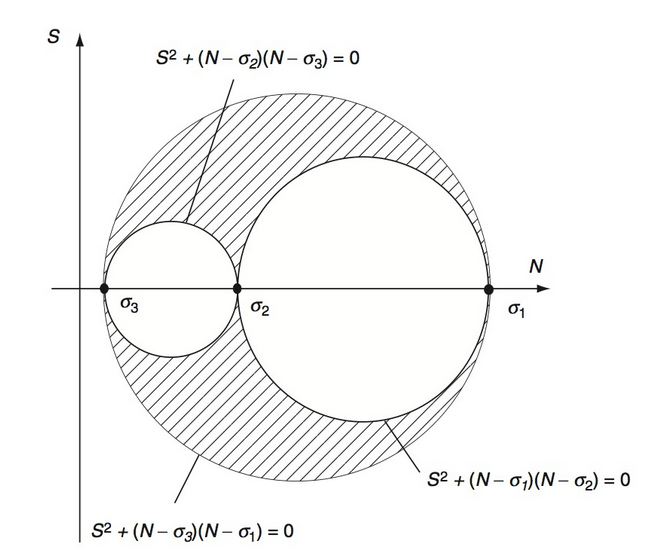
\includegraphics{../images/mohr.PNG}
\end{frame}

\hypertarget{material-behavior}{%
\section{material behavior}\label{material-behavior}}

\begin{frame}{topics}
\protect\hypertarget{topics-1}{}
\begin{itemize}
\tightlist
\item
  Hooke's Law
\item
  Physical meaning of elastic constants
\item
  Thermal expansion
\end{itemize}
\end{frame}

\begin{frame}{hooke's law}
\protect\hypertarget{hookes-law}{}
\begin{itemize}
\tightlist
\item
  Can be written in terms of strain
\end{itemize}

\[\epsilon_{ij} = \frac{1+\nu}{E}\sigma_{ij} - \frac{\nu}{E}\sigma_{kk} \delta_{ij}\]

\begin{itemize}
\tightlist
\item
  Or stress
\end{itemize}

\[\sigma_{ij} = \lambda \epsilon_{kk}\delta_{ij} + 2\mu \epsilon_{ij}\]
\end{frame}

\begin{frame}{physical meaning}
\protect\hypertarget{physical-meaning}{}
\begin{itemize}
\tightlist
\item
  Young's modulus
\item
  Poisson's ratio
\item
  Shear modulus
\item
  Bulk modulus
\end{itemize}
\end{frame}

\begin{frame}{thermoelasticity}
\protect\hypertarget{thermoelasticity}{}
\begin{itemize}
\tightlist
\item
  Separate strain into mechanical and thermal components
\end{itemize}

\[\epsilon_{ij} = \epsilon_{ij}^M + \epsilon_{ij}^T\]

\begin{itemize}
\tightlist
\item
  For isotropic materials:
\end{itemize}

\[\epsilon_{ij} = \alpha (T - T_0)\delta_{ij}\]
\end{frame}

\begin{frame}{thermoelasticity}
\protect\hypertarget{thermoelasticity-1}{}
\begin{itemize}
\tightlist
\item
  We can combine this with Hooke's Law to find
\end{itemize}

\[\epsilon_{ij} = \frac{1+\nu}{E}\sigma_{ij} -\frac{\nu}{E}\sigma_{kk}\delta_{ij} + \alpha (T-T_0)\delta_{ij}\]

\begin{itemize}
\tightlist
\item
  Or formulated in terms of stress (and Lamé constants)
\end{itemize}

\[\sigma_{ij} = \lambda \epsilon_{kk} \delta_{ij} + 2\mu \epsilon_{ij} - (3\lambda + 2\mu) \alpha (T - T_0) \delta_{ij}\]
\end{frame}

\hypertarget{problem-formulation}{%
\section{problem formulation}\label{problem-formulation}}

\begin{frame}{topics}
\protect\hypertarget{topics-2}{}
\begin{itemize}
\tightlist
\item
  Boundary conditions
\item
  Compatibility
\item
  Beltrami-Michell
\item
  Navier's Equations
\item
  Superposition
\end{itemize}
\end{frame}

\begin{frame}{boundary conditions}
\protect\hypertarget{boundary-conditions}{}
\begin{itemize}
\tightlist
\item
  Traction
\item
  Displacement
\item
  Mixed
\end{itemize}
\end{frame}

\begin{frame}{compatibility}
\protect\hypertarget{compatibility}{}
\begin{itemize}
\tightlist
\item
  If continuous, single-valued displacements are specified,
  differentiation will result in well-behaved strain field
\item
  The inverse relationship, integration of a strain field to find
  displacement, may not always be true
\item
  There are cases where we can integrate a strain field to find a set of
  discontinuous displacements
\end{itemize}
\end{frame}

\begin{frame}{compatibility}
\protect\hypertarget{compatibility-1}{}
\begin{itemize}
\tightlist
\item
  The compatibility equations enforce continuity of displacements to
  prevent this from occurring
\item
  To enforce this condition we consider the strain-displacement
  relations:
\end{itemize}

\[\epsilon_{ij} = \frac{1}{2}(u_{i,j} + u_{j,i})\]

\begin{itemize}
\tightlist
\item
  and differentiate with respect to \(x_k\) and \(x_l\)
\end{itemize}

\[\epsilon_{ij,kl} = \frac{1}{2}(u_{i,jkl} + u_{j,ikl})\]

\begin{itemize}
\tightlist
\item
  Or
\end{itemize}

\[2\epsilon_{ij,kl} = u_{i,jkl} + u_{j, ikl}\]
\end{frame}

\begin{frame}{compatibility}
\protect\hypertarget{compatibility-2}{}
\begin{itemize}
\tightlist
\item
  We can eliminate the displacement terms from the equation by
  interchanging the indexes to generate new equations
\end{itemize}

\[\begin{aligned}
    2\epsilon_{ik,jl} &= u_{i,jkl} + u_{k,ijl} \\
    2\epsilon_{jl,ik} &= u_{j,ikl} + u_{l,ijk}
\end{aligned}\]

\begin{itemize}
\tightlist
\item
  Solving for \(u_{i,jkl}\) and \(u_{j,ikl}\)
\end{itemize}

\[\begin{aligned}
    u_{i,jkl} &= 2\epsilon_{ik,jl} - u_{k,ijl} \\
    u_{j,ikl} &= 2\epsilon_{jl,ik} - u_{l,ijk}
\end{aligned}\]
\end{frame}

\begin{frame}{compatibility}
\protect\hypertarget{compatibility-3}{}
\begin{itemize}
\tightlist
\item
  Substituting these values into the equations gives
\end{itemize}

\[2\epsilon_{ij,kl} = 2\epsilon_{ik,jl} - u_{k,ijl} + 2\epsilon_{jl,ik} - u_{l, ijk}\]

\begin{itemize}
\tightlist
\item
  We now consider one more change of index equation
\end{itemize}

\[2\epsilon_{kl,ij} = u_{k,ijl} + u_{l,ijk}\]

\begin{itemize}
\tightlist
\item
  and substituting this result gives
\end{itemize}

\[2\epsilon_{ij,kl} = 2\epsilon_{ik,jl} + 2\epsilon_{jl,ik} - 2\epsilon_{kl,ij}\]

\begin{itemize}
\tightlist
\item
  Or, simplified
\end{itemize}

\[\epsilon_{ij,kl} + \epsilon_{kl,ij} - \epsilon_{ik,jl} - \epsilon_{jl,ik} = 0\]
\end{frame}

\begin{frame}{beltrami-michell}
\protect\hypertarget{beltrami-michell}{}
\begin{itemize}
\tightlist
\item
  When working with stress functions, it is convenient to check
  compatibility of the stress function directly
\item
  Using Hooke's Law, we can formulate compatibility in terms of stress
\item
  These are known as the Beltrami-Michell equations
\end{itemize}
\end{frame}

\begin{frame}{navier's equations}
\protect\hypertarget{naviers-equations}{}
\begin{itemize}
\tightlist
\item
  Similarly, we can write the equilibrium equations in terms of
  displacement
\item
  This is convenient when dealing with displacement boundary conditions
\item
  Known as Navier's equations
\end{itemize}
\end{frame}

\end{document}
